% results.tex
\chapter{Results}

\section*{Genome Interaction Scaling}
We mapped the reads to the genome as described in the Methods.  Upon mapping reads to interaction matrices, we noted that the number
of observed interactions per bin scales differently by chromosome.  We plotted the percentage of reads observed for each chromosome
in 1Mb bins (Figure~\ref{fig:probeScalesMb}) and by percentage of chromosome length (Figure~\ref{fig:probeScalesPercent}).

\begin{figure}[H]
  \caption{Chromosome Contact Scaling}
  \noindent%
  \begin{minipage}[b]{0.45\textwidth}\label{fig:probeScalesMb}
    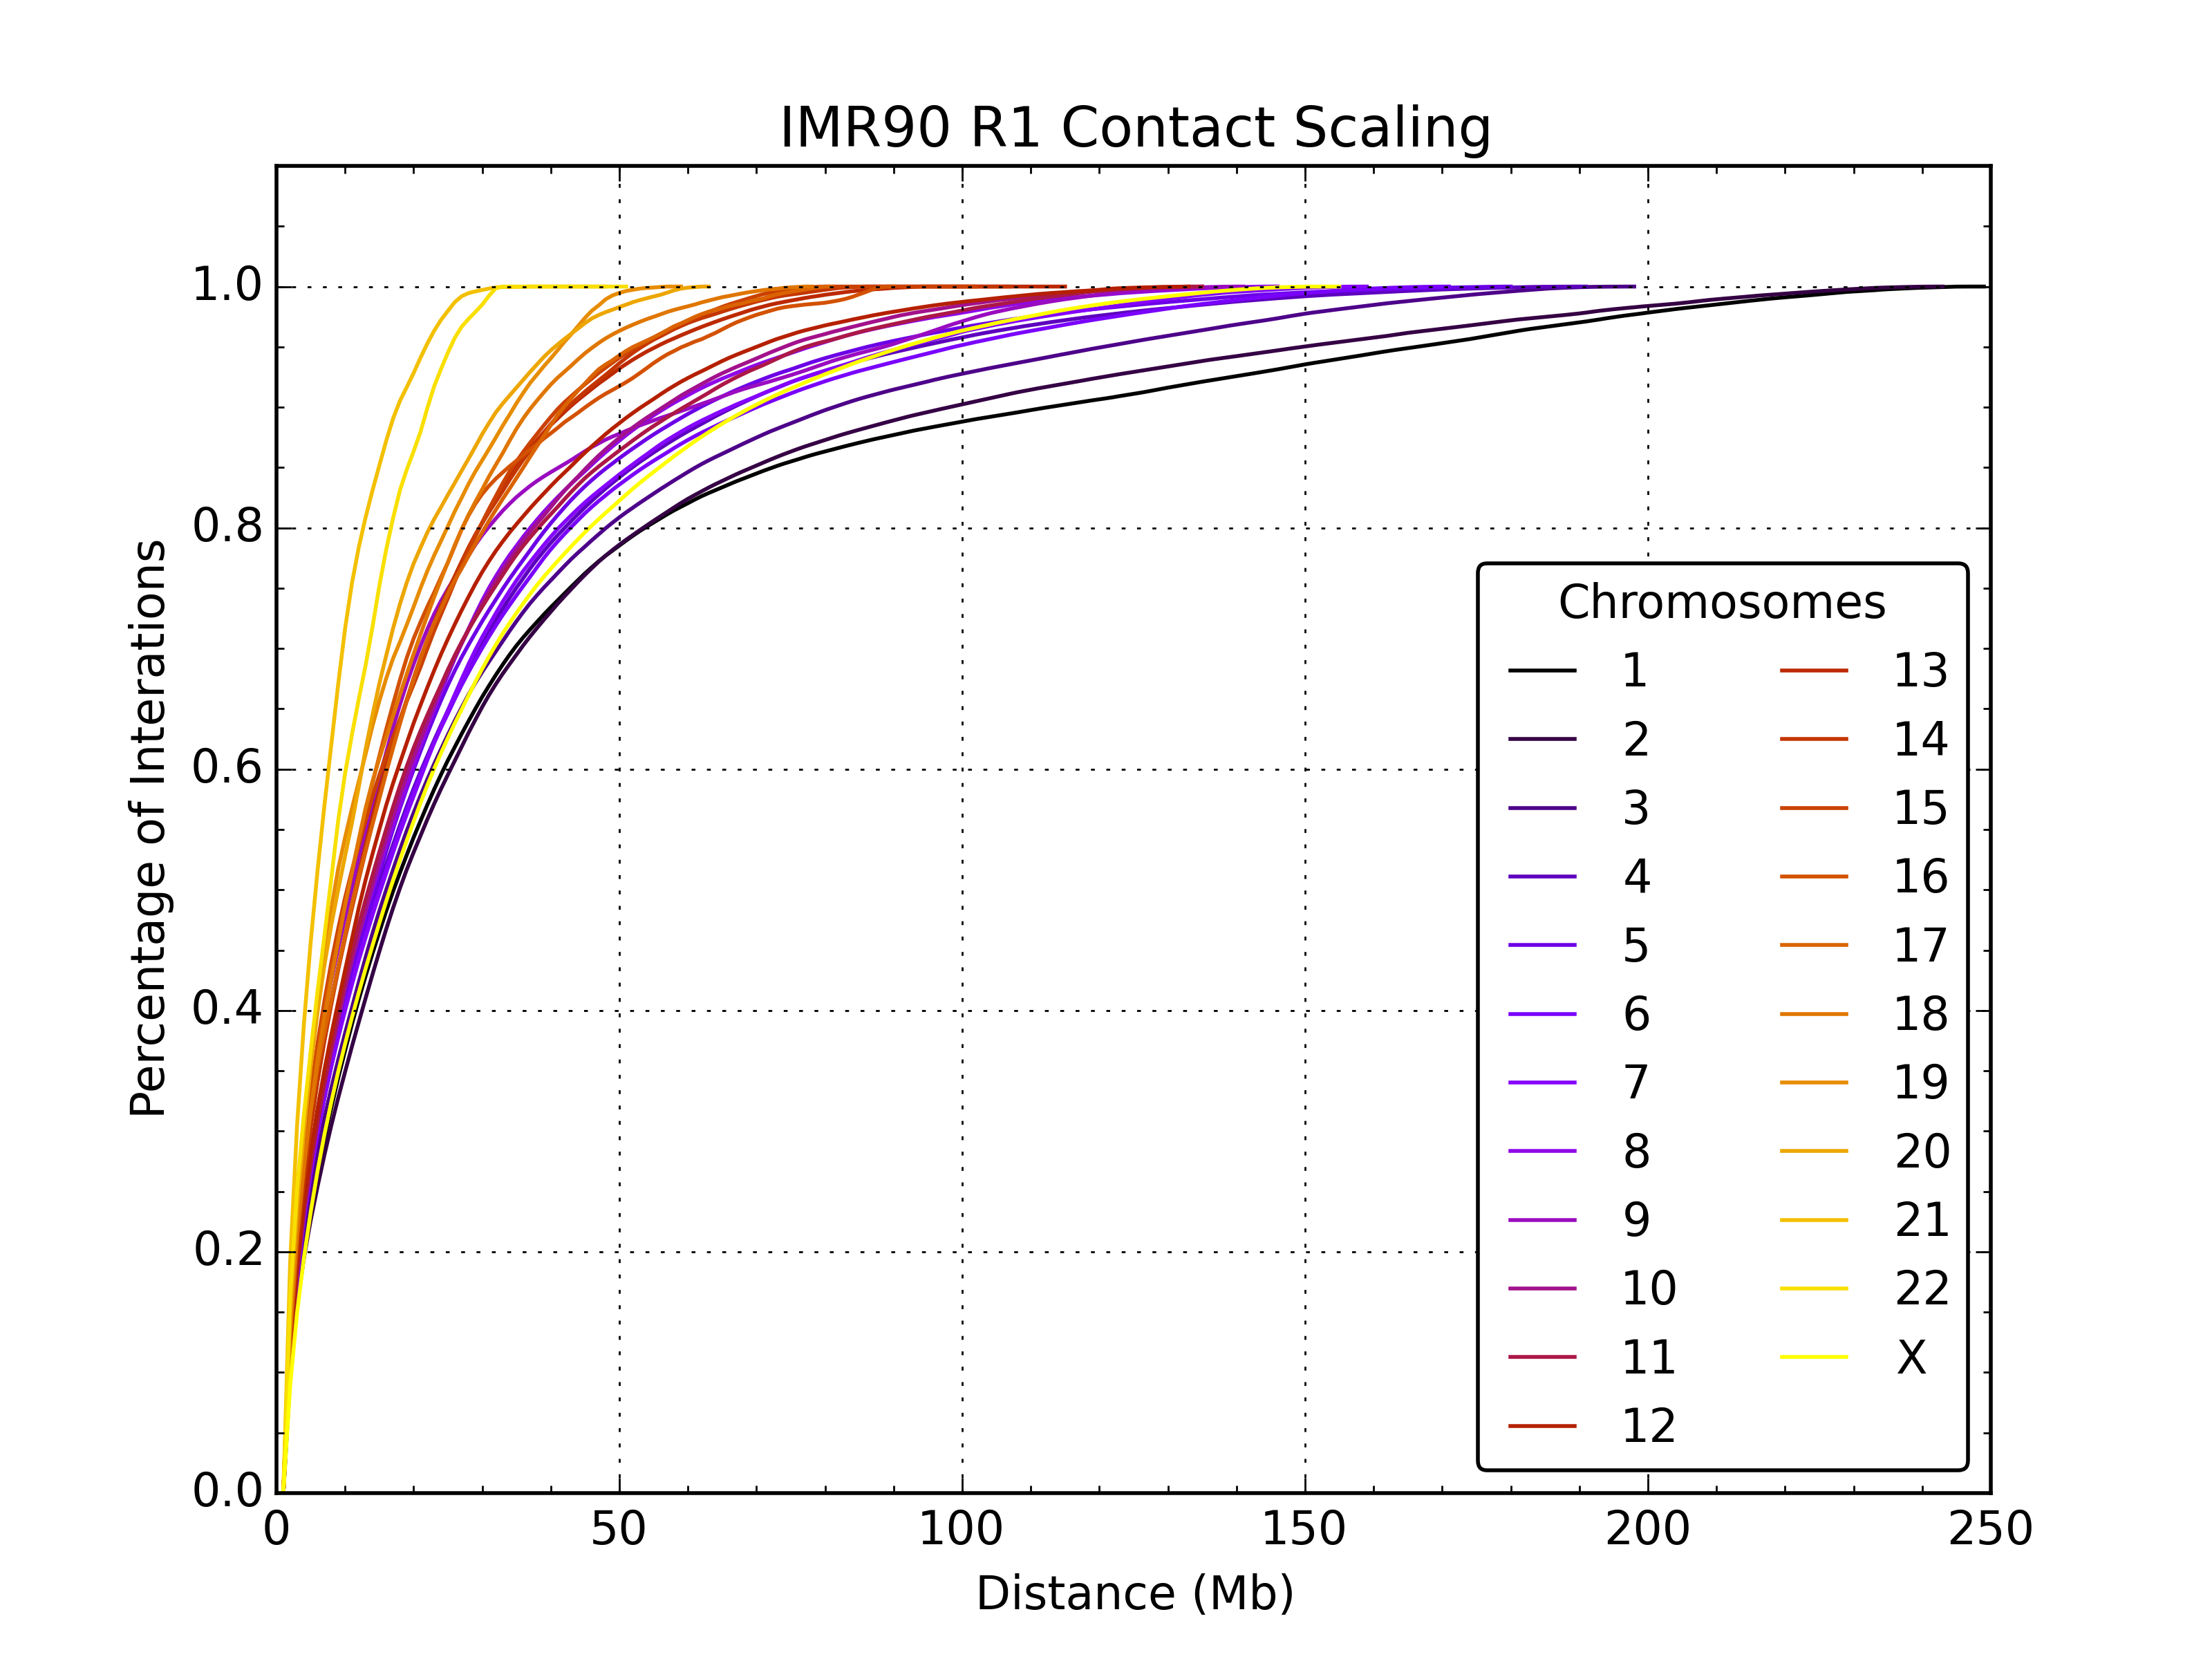
\includegraphics[width=\linewidth]{./figures/results/probeScalesMb.png}
  \end{minipage}%
  \hfill
  \begin{minipage}[b]{0.45\linewidth}\label{fig:probeScalesPercent}
    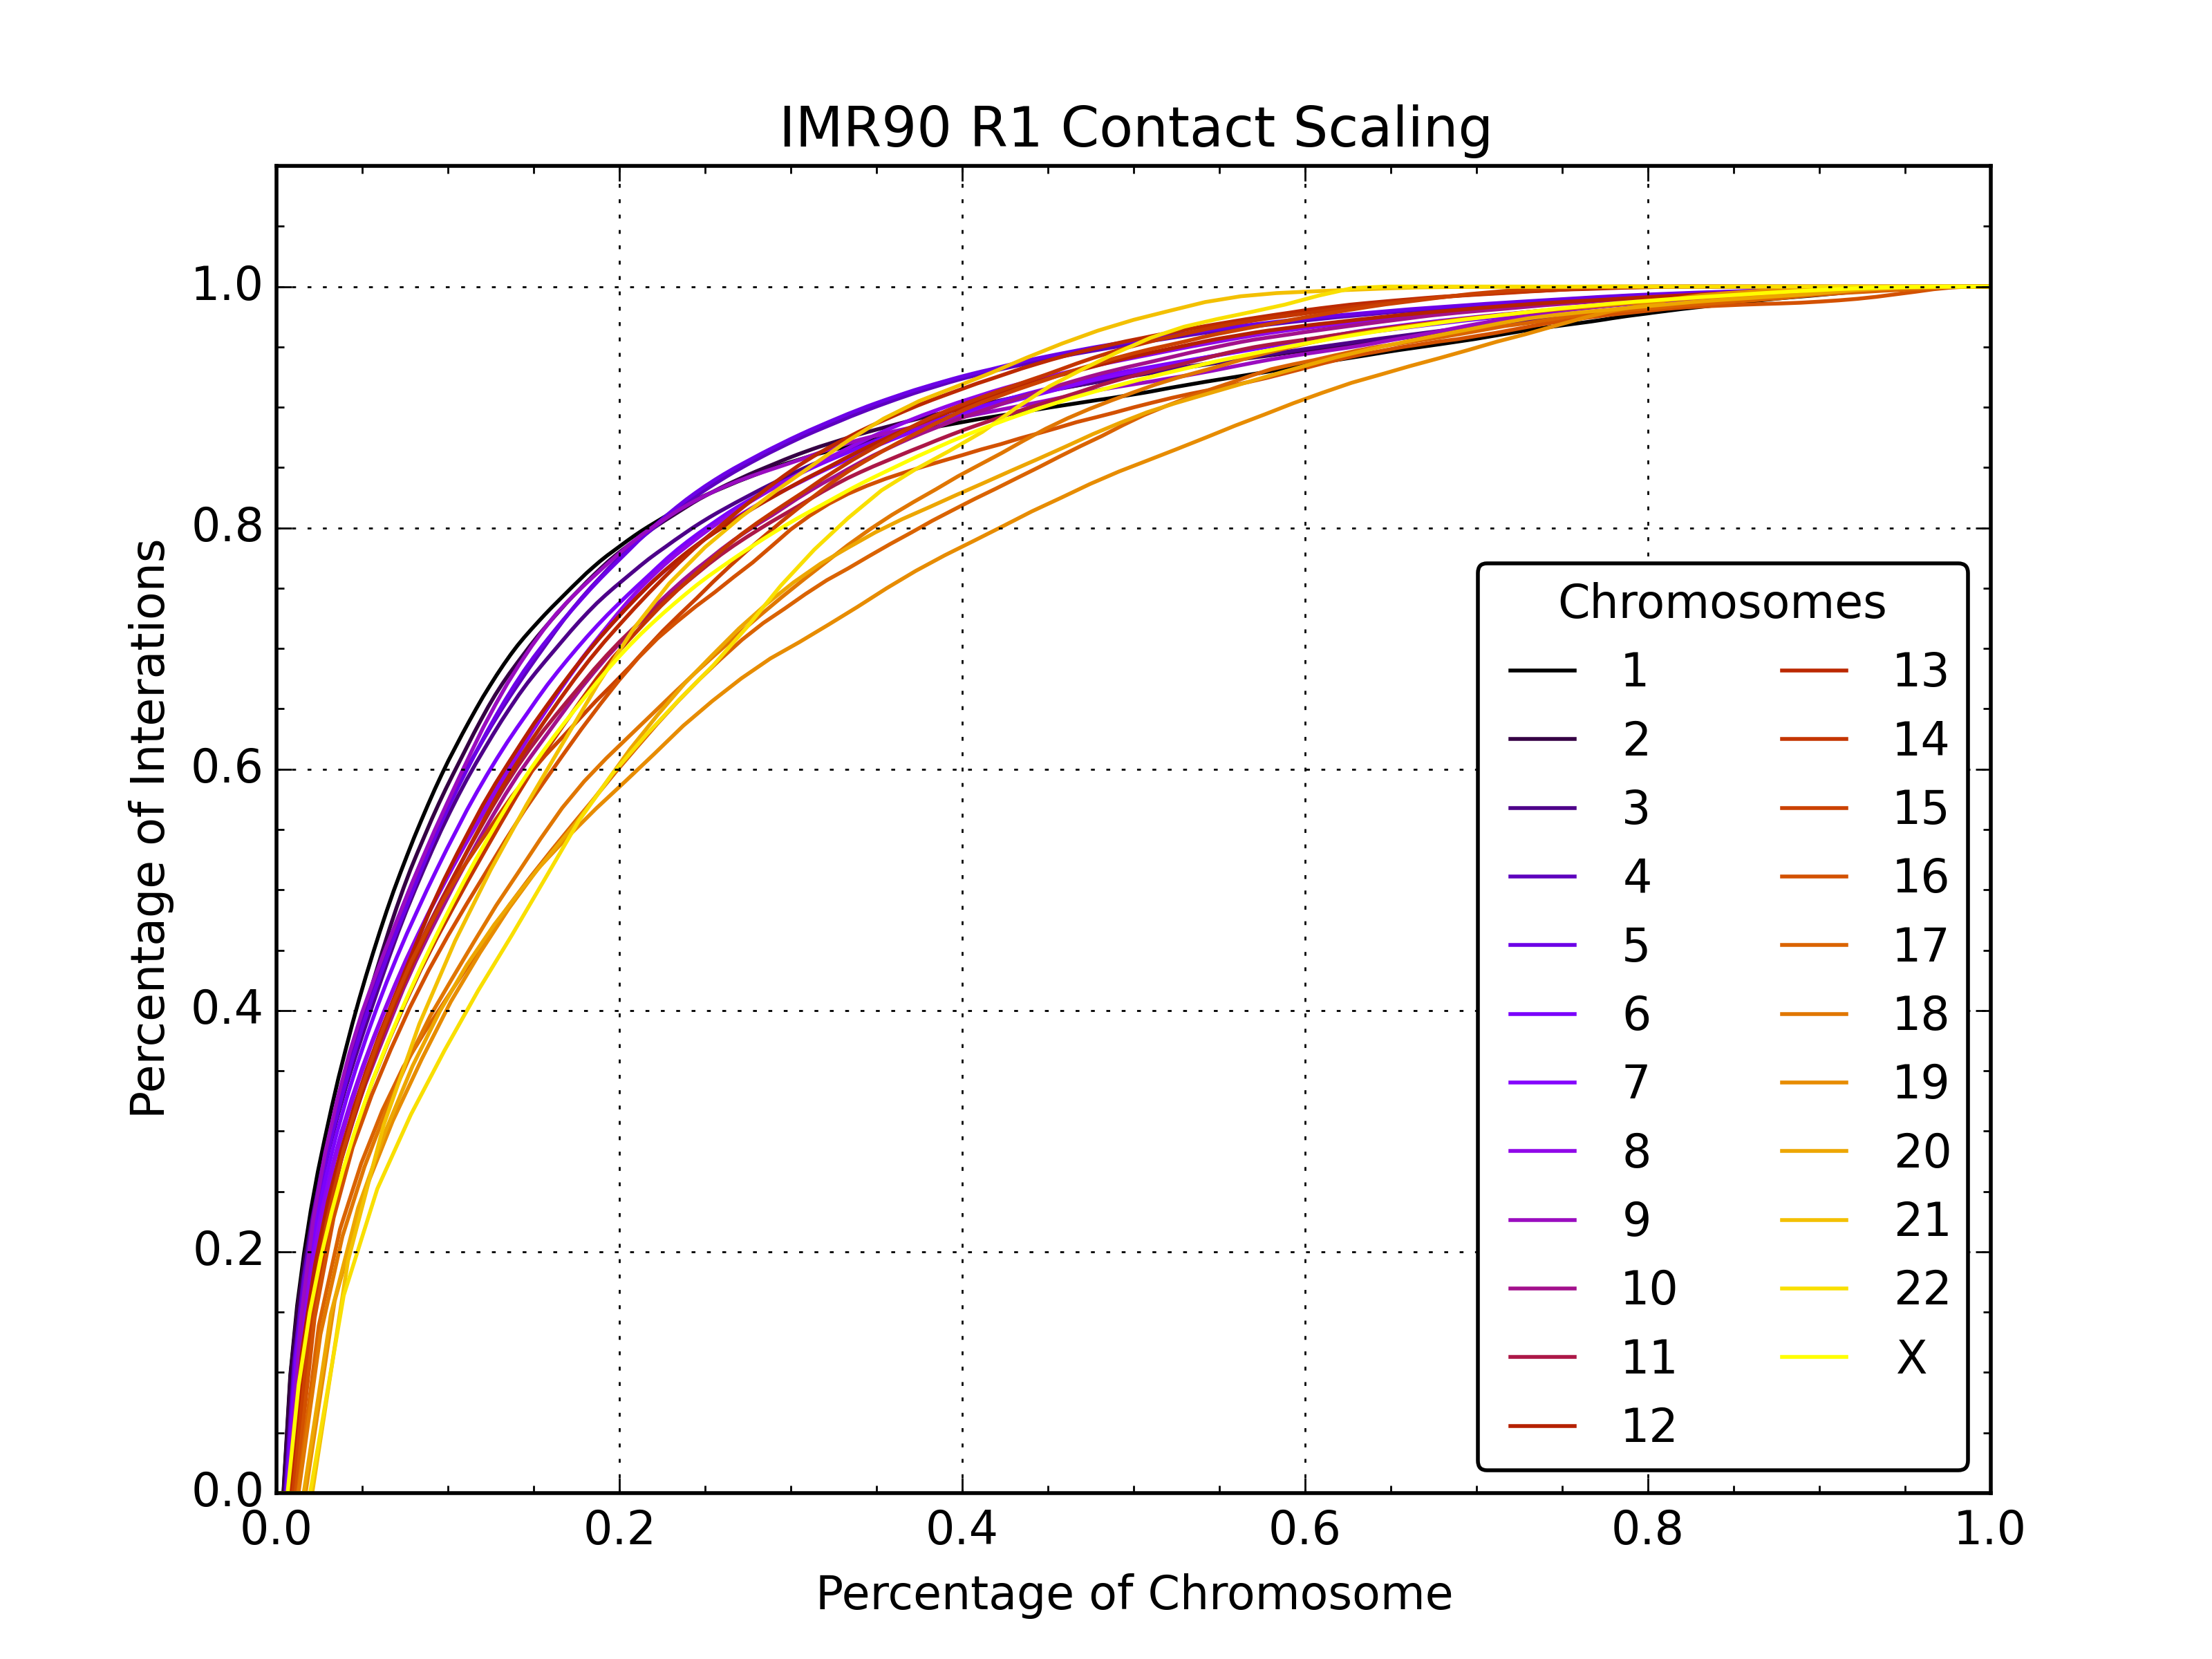
\includegraphics[width=\textwidth]{./figures/results/probeScalesPercent.png}
  \end{minipage}
\end{figure}

We remarked that chromosomes have heterogeneous scaling properties.  We examined the character of the chromosome for all replicates
by computing the coordinate at which we observed $50\%$ of the total chromosome contacts.  These finding are shown below (Figure~\ref{fig:probeCom}).

\begin{figure}[H]
  \centering
  \caption{Chromosome Interaction Half-Max}\label{fig:probeCom}
  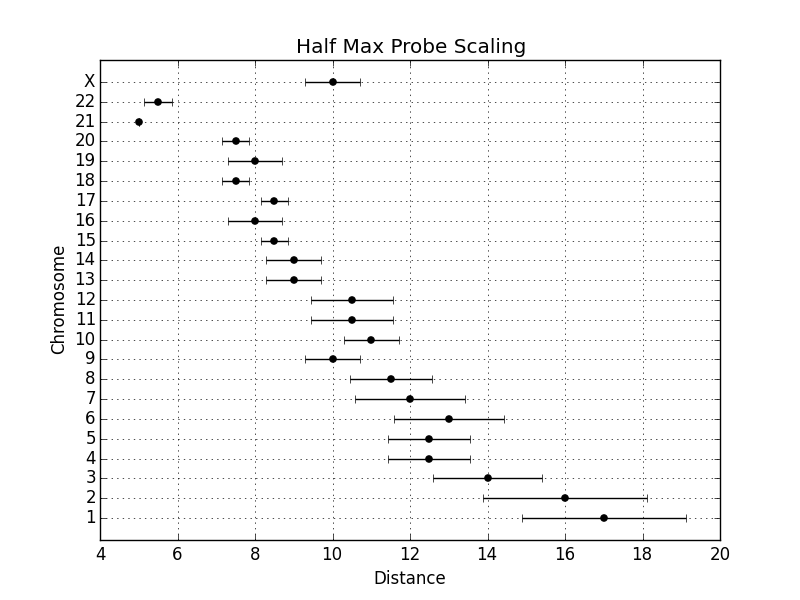
\includegraphics[width=\textwidth]{./figures/results/com.png}
  \medskip
  \small
  Intra-chromosomal interactions are considered for each chromosome across all replicates.  For the entire chromosome, the average number of
  contacts at a given genomic distance was calculated using Equation~\ref{eq:probeScale}.  For each replicate, the distance at which the number
  of contacts exceeded one half the total number of contacts for that chromosome was determined.  The mean and standard error of the half max
  is plotted above for each chromosome in IMR90.
\end{figure}

\section*{Eigenvector Partitioning of Chromatin Compartments}

We tested whether a change in the compartment character (measured by the principal component) plays a significant role in regulation
by plotting and computing correlations between the eigenvector and gene expression.  Using replicated IMR90 and hESC \gls{mRNA} expression
experiments, we plotted changes in gene expression against the gene's compartment character in IMR90 (Figure~\ref{fig:expressionChangeByCompartment}).
We also considered the change between compartments character against gene expression levels, finding no significant correlation ($\rho = -0.01$,
$p$-value negligible. See Figure~\ref{fig:expressionChangeByCompartmentChange}).

\begin{figure}[H]
  \caption{Gene Expression Change by Compartment Change}
  \begin{minipage}[b]{0.45\textwidth}\label{fig:expressionChangeByCompartmentChange}
    \includegraphics[width=\textwidth]{./figures/results/volcano.png}
  \end{minipage}%
  \hfill
  \begin{minipage}[b]{0.45\textwidth}\label{fig:expressionChangeByCompartment}
    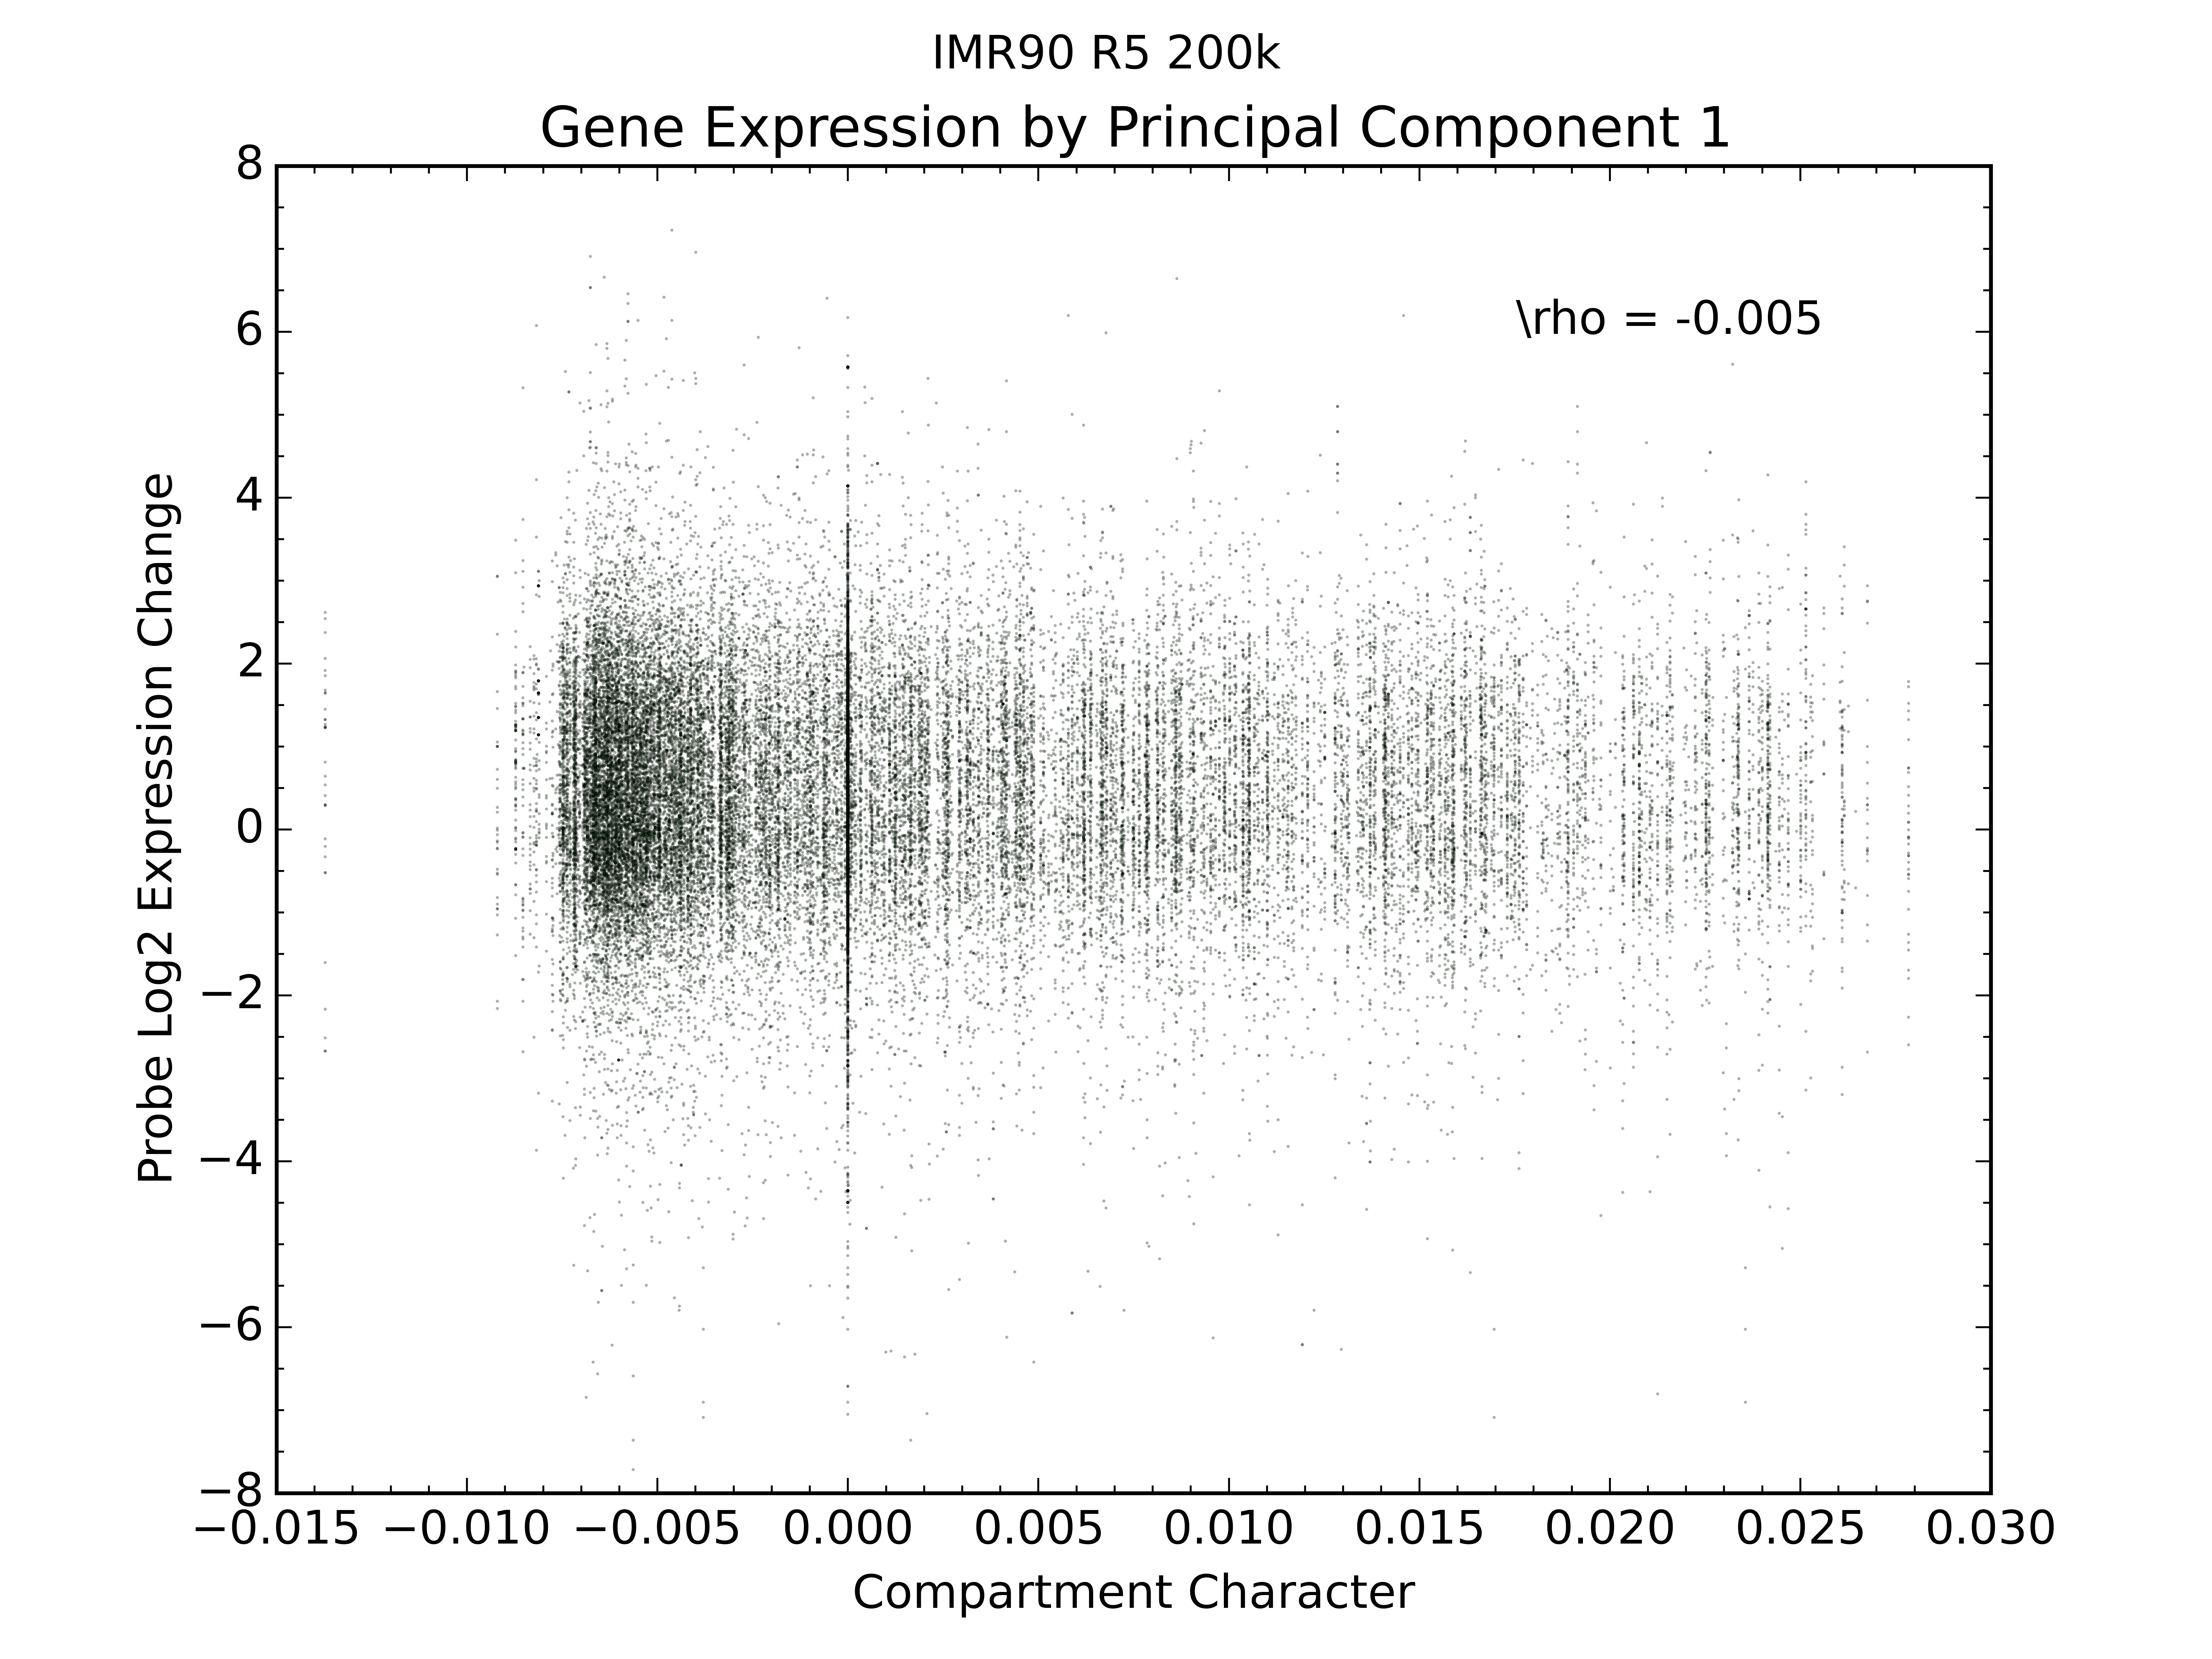
\includegraphics[width=\textwidth]{./figures/results/compartment_ir5_200k.png}
  \end{minipage}
\end{figure}

We asked if \gls{CFS} were enriched in a given compartment.  We computed the compartment character from the first \gls{PC} across fragile
sites, displaying them in a histogram.  The fragile sites were evenly distributed between nuclear compartments (Figure~\ref{fig:compartmentCFS}).

\begin{figure}[H]
  \centering
  \caption{Fragile Sites in Compartments}\label{fig:compartmentCFS}
  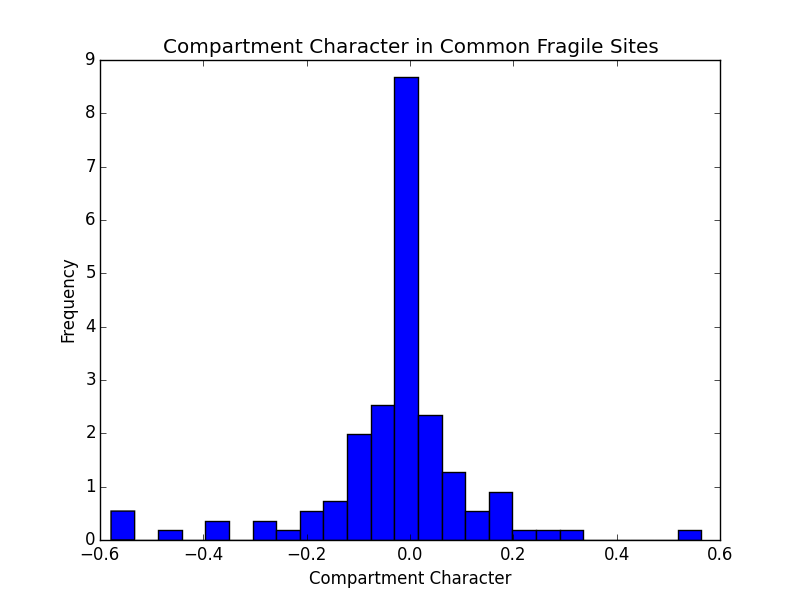
\includegraphics[width=\textwidth]{./figures/results/cfs.png}
\end{figure}

\section*{Directionality Indices}

If the nuclear architecture can be decomposed into layers as we have hypothesized, topological domains may exist at different
scales or resolutions within the nucleus.  We tested this hypothesis by calculating directionality indices at various window sizes
on a high resolution contact map.  Interestingly, we found that the minimum correlations between indices at a given window size increased
with higher resolution map ($\rho_{\min}(100kb) = 0.77, \rho_{\min}(1Mb) = 0.70$, Supplementary Information~\ref{sec:SuppDirectionality}).

\section*{Domain Discovery}

Previous discovered domains show enrichment in chromatin modeling proteins, housekeeping genes, and retrotransposons at the topological domain
boundaries \citep{dixon2012}.  We used a naive heuristic to discover conserved topological domain sets at smaller resolutions than previously reported.

\begin{figure}[H]
  \caption{Number of Domains by Chromosome}
  \begin{minipage}{0.45\textwidth}%
    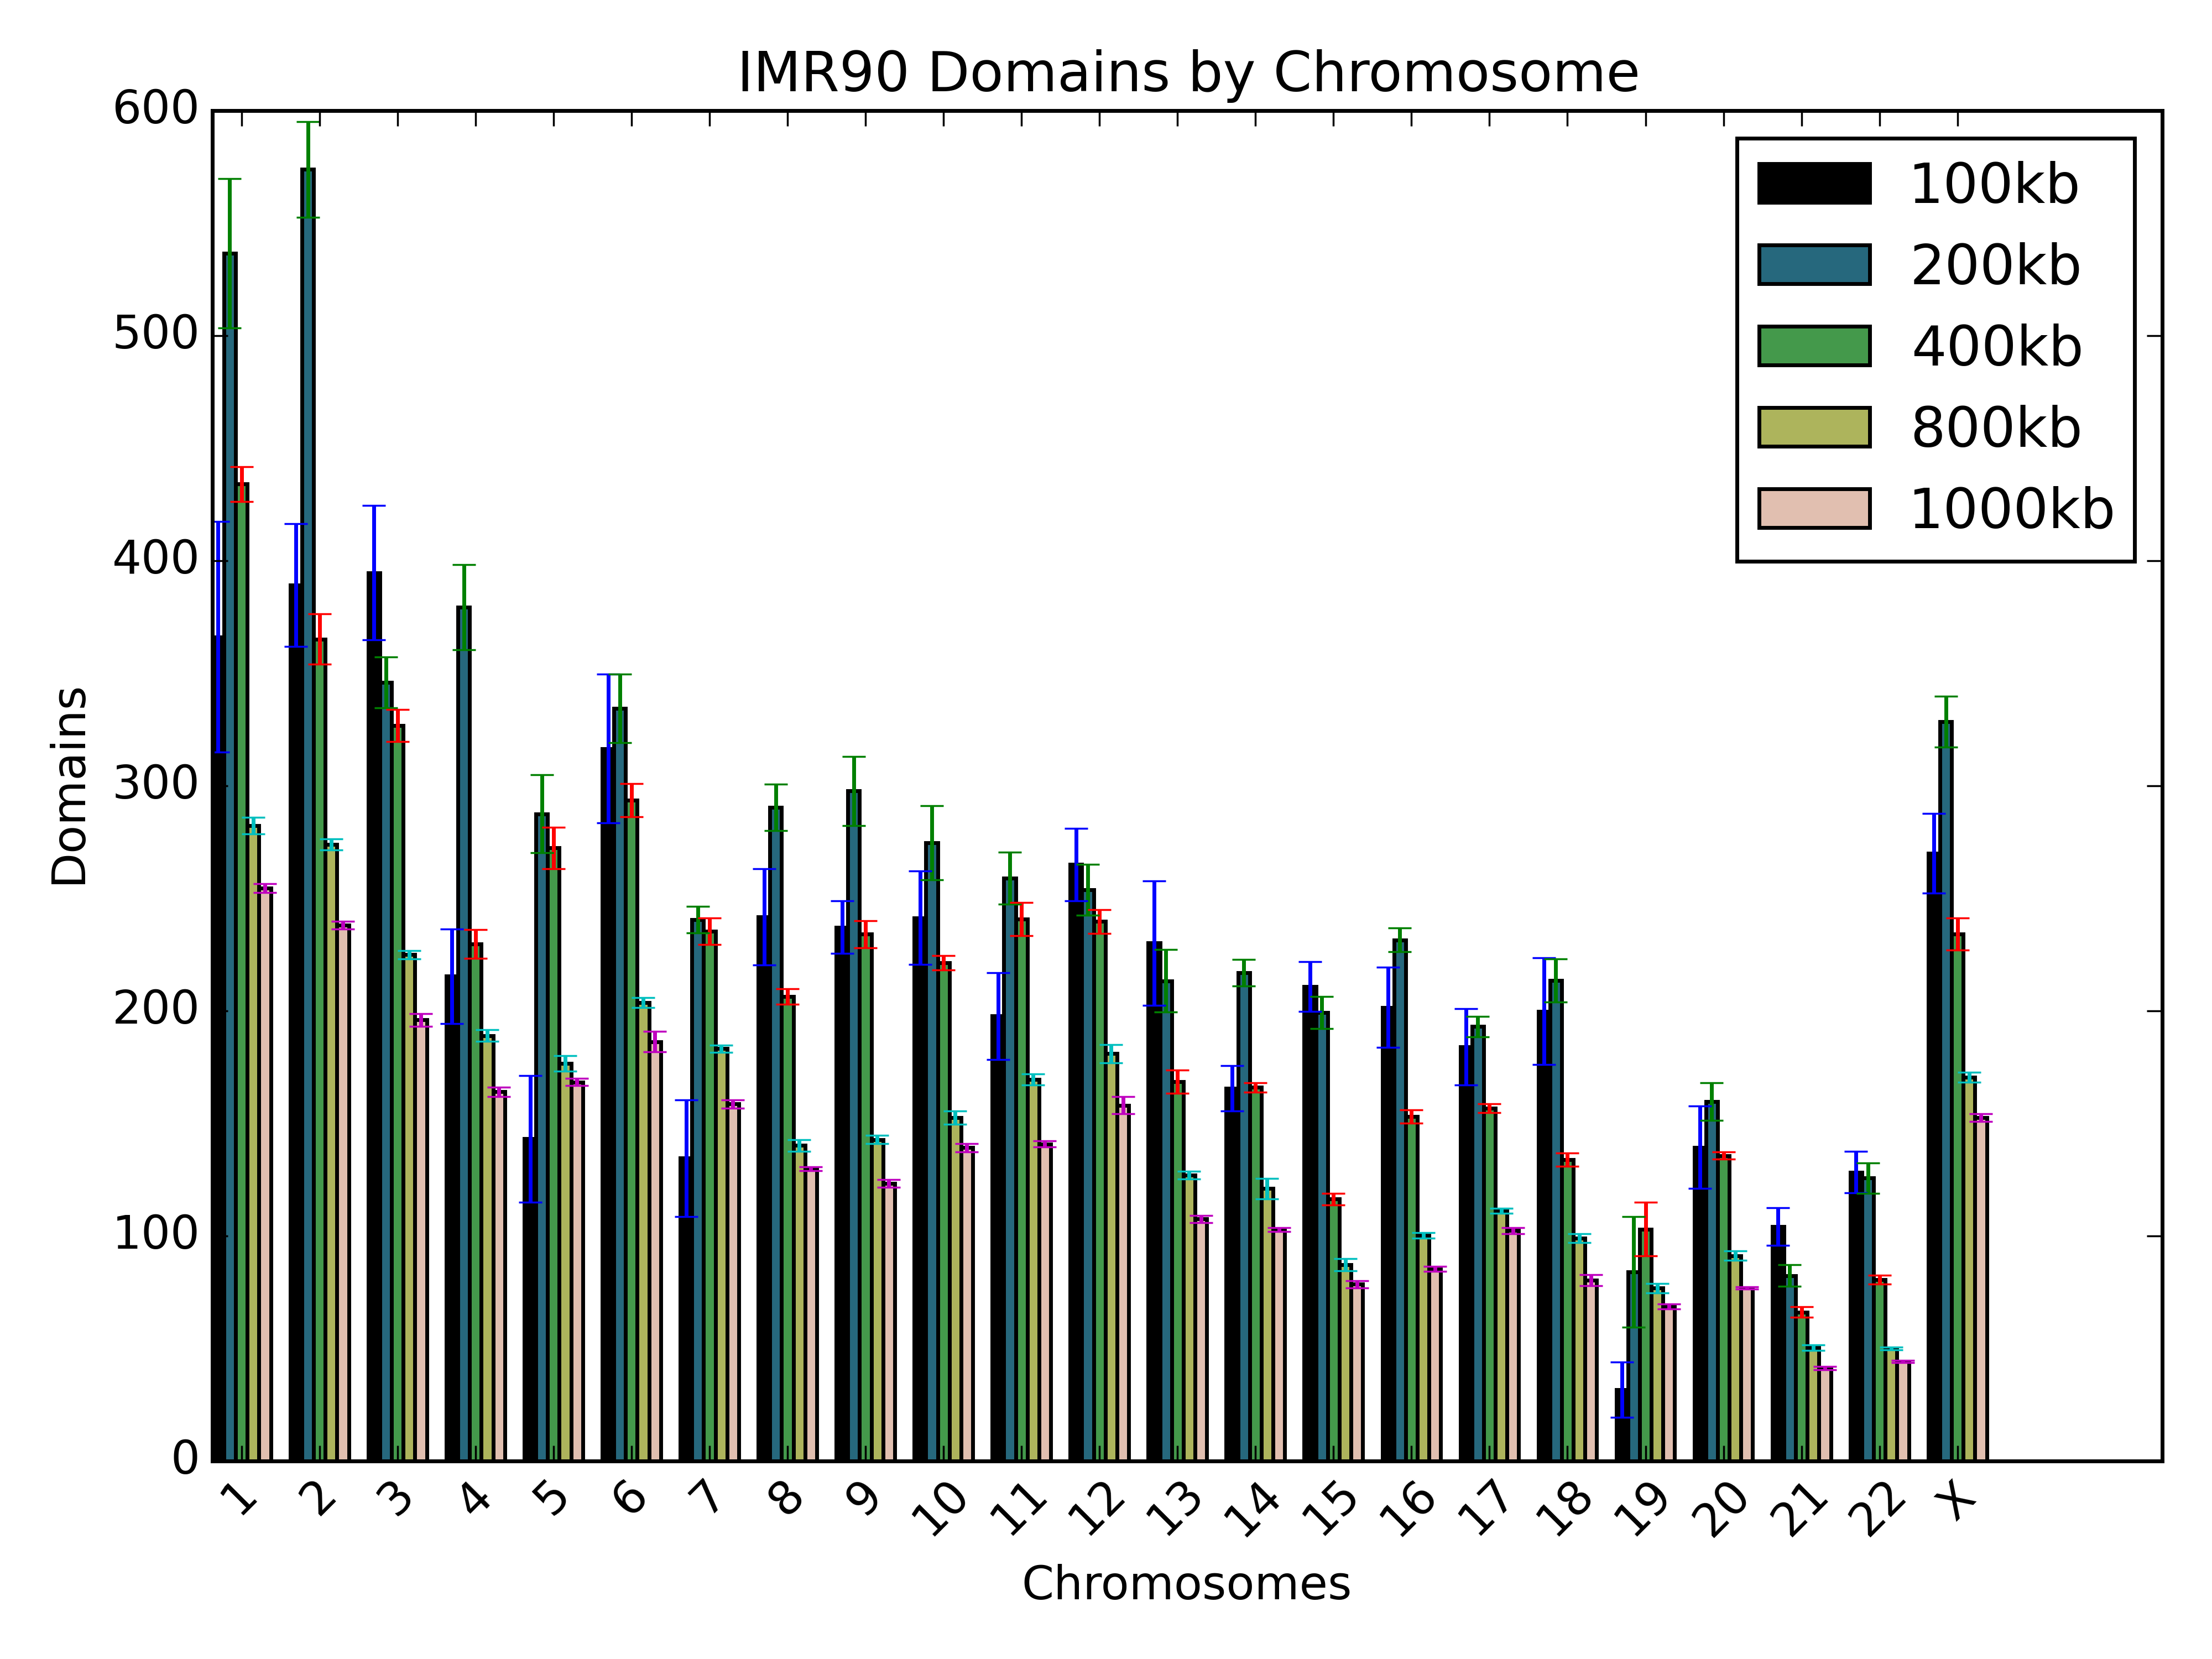
\includegraphics[width=\textwidth]{./figures/results/domain_imr90_bar.png}
  \end{minipage}%
  \hfill
  \begin{minipage}{0.45\textwidth}
    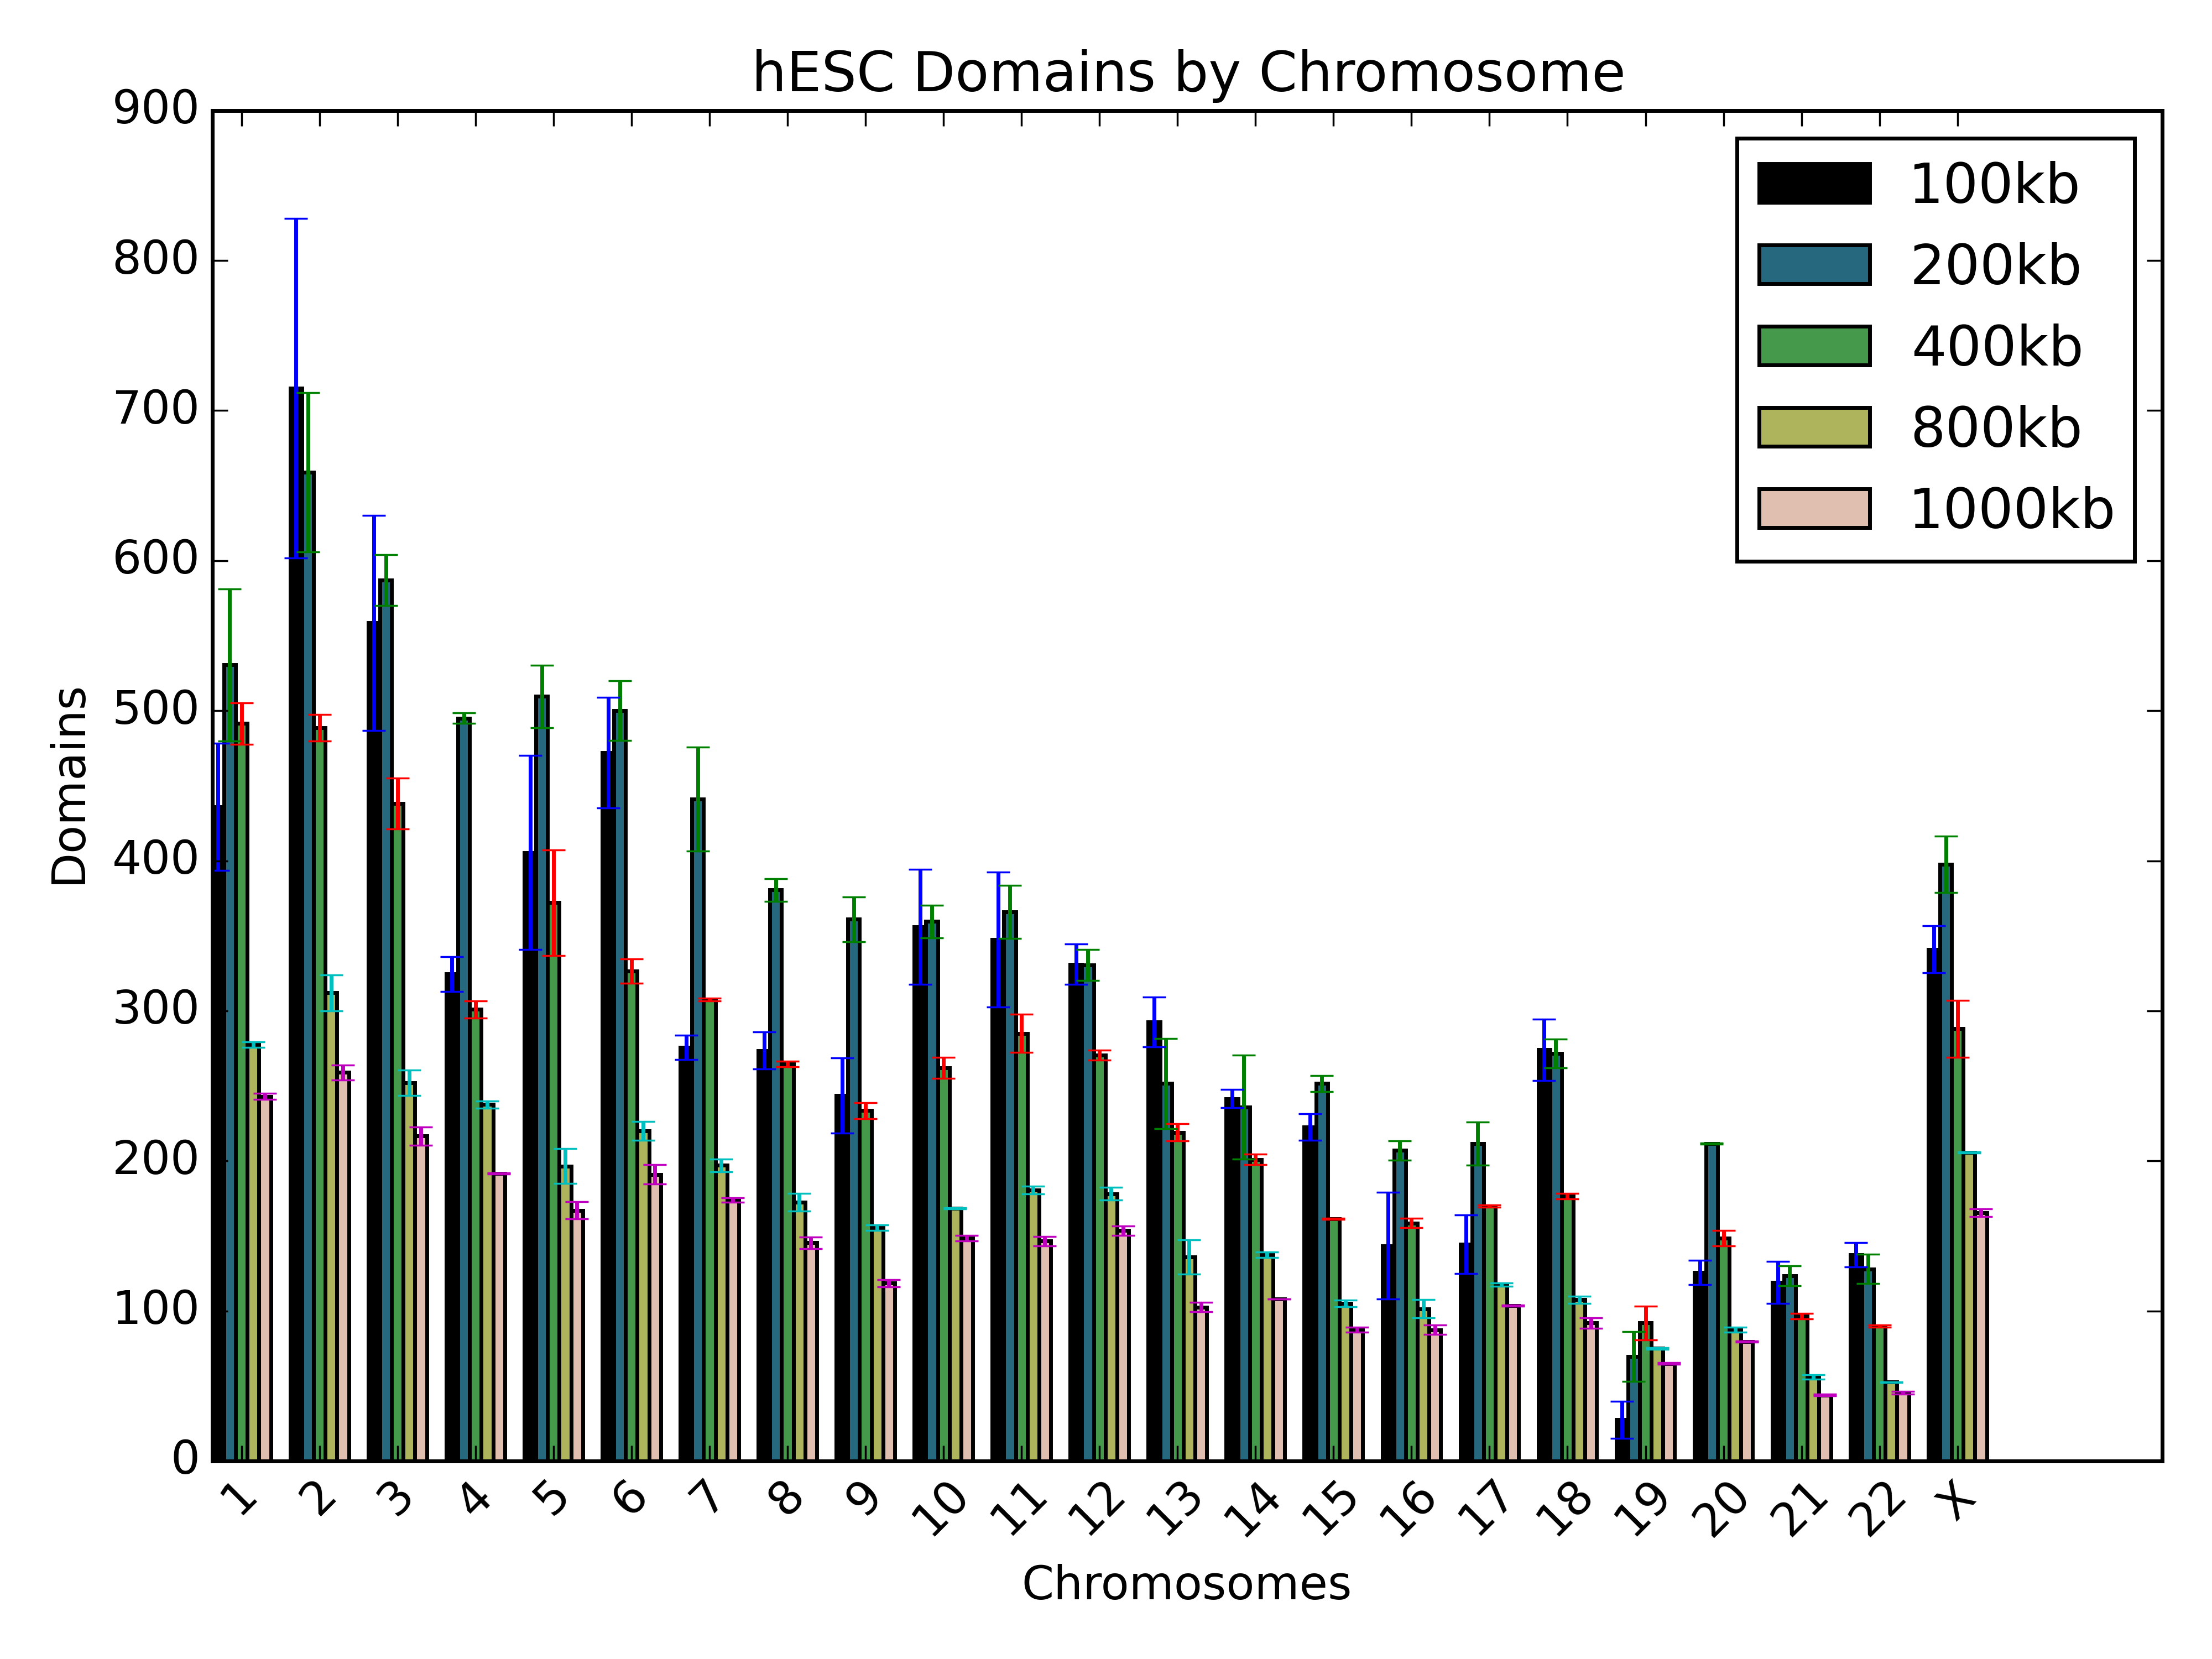
\includegraphics[width=\textwidth]{./figures/results/domain_hesc_bar.png}
  \end{minipage}
\end{figure}

We computed domains using DI window sizes as 10kb
